\documentclass[a4paper,11pt]{article}

\usepackage[french]{babel}
\usepackage[T1]{fontenc}
\usepackage[utf8]{inputenc}
\usepackage{lmodern}
\usepackage{microtype}
\usepackage{graphicx}
\usepackage{subcaption}

\usepackage{hyperref}
\usepackage[margin=1in]{geometry} %Change la marge
\usepackage{xurl}

\title{TIPE : Mis à jour du projet et avancées}
\author{DE CARVALHO Enzo et ALEXANDRINE Pedro}

\begin{document}
\maketitle
\section{Motivations : rappels}
	Le but est de modéliser, à l'aide de machine learning, l'évolution des 
	chiffres liès (à priori ici, les décès) et si possible, d'affiner la 			modélisation pour mieux prédir l'évolution de la courbe, et/ou étudier 			les limites de la modélisation

\section{Résultats et avancées actuelles}
	Nous avons alors, dans un premier lieu réalisé différentes regressions
	linéaire à l'aide du package \texttt{sklearn} en python proposant déjà
	

\begin{figure}[h!]
  \centering
  \begin{subfigure}[b]{0.5\linewidth}
    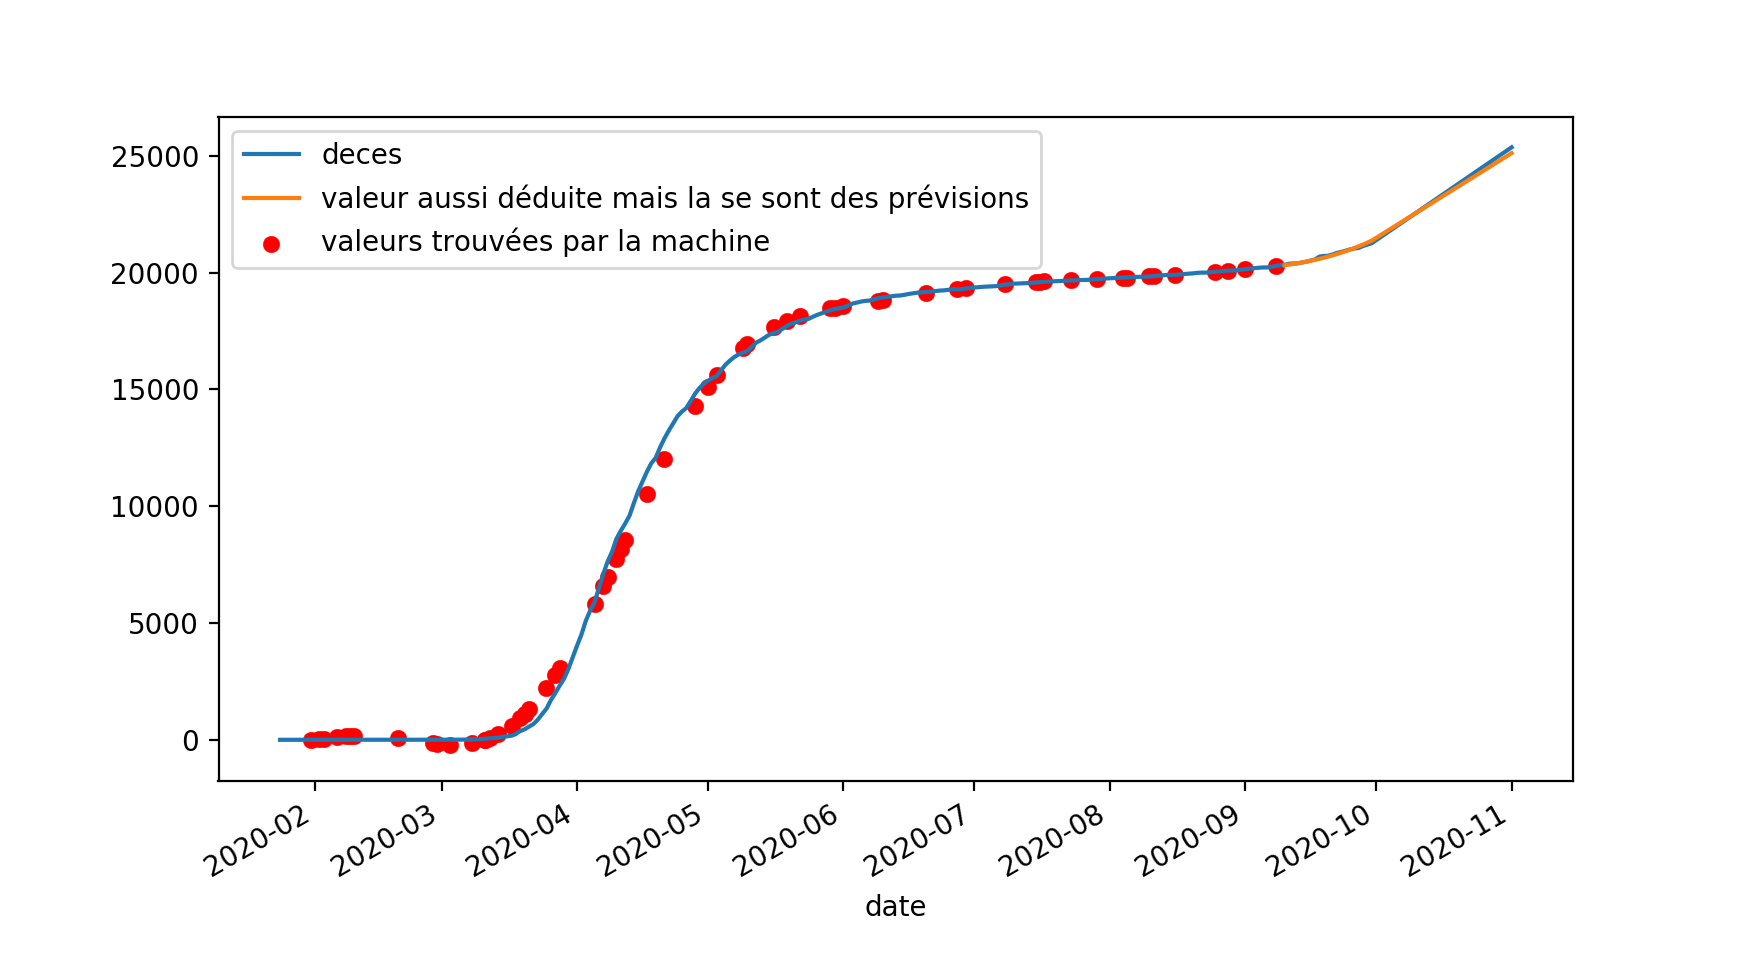
\includegraphics[width=\linewidth]{deces_covid_machinelearning1.png}
   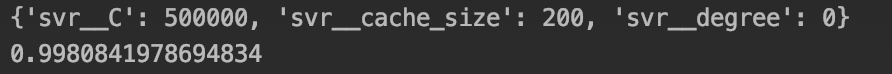
\includegraphics[width=\linewidth]{params1.png}
    \caption{premier test SVR et paramètre }
     \end{subfigure}
  \begin{subfigure}[b]{0.5\linewidth}
    \includegraphics[width=\linewidth]{Test prévision elasticNet.png}
   \includegraphics[width=\linewidth]{paramètre test ElasticNet.pdf}
    \caption{premier test SVR et paramètre }
  \end{subfigure}
  \caption{Test de prévision avec régression}
  \label{fig:coffee}
\end{figure}








	
\end{document}